\documentclass[12pt,letterpaper,boxed]{math_hw_pset}
\usepackage[margin=1in]{geometry}
\usepackage{graphicx}
\usepackage{bm}
\usepackage{amsmath} 
\usepackage{braket} 
\usepackage{relsize}
\usepackage{lmodern} % math, rm, ss, tt
\usepackage[T1]{fontenc}
\usepackage{fancyhdr}
\usepackage{hyperref}
\newcommand{\zz}{\mathbb{Z}}
\newcommand{\rr}{\mathbb{R}}
\newcommand{\nn}{\mathbb{N}}
\newcommand{\qq}{\mathbb{Q}}
\newcommand*{\ms}[1]{\ensuremath{\mathscr{#1}}}
\renewcommand{\labelenumi}{{\bf (\alph{enumi})}}
\renewcommand{\epsilon}{\varepsilon}
\newcommand{\oo}{\mathcal{O}}

\pagestyle{fancy}
\fancyhf{}
\rhead{Spring 2020}
\lhead{\vspace{5mm} Math 143}
\rfoot{Page \thepage}
\chead{Homework \# 4}


% info for header block in upper right hand corner
\name{Name: Luke Trujillo}
\duedate{Due Date: 3/220} 

\begin{document}
\begin{center}
    143 Hw \# 4
\end{center}

\begin{exercise}[Problem 1.]
    Find two recent ML papers (from 2016 to now) and the corresponding GitHub code which use at least one of the following: 
    (Riemannian) connections, parallel transport, covariant derivatives, and geodesics on manifold.  
    Then study one of the papers in details and make the code running to generate figures in the paper.
\end{exercise}

\begin{solution}
    The two papers I decided to look at are: 
    \begin{itemize}
        \item \href{https://arxiv.org/pdf/1807.07258v2.pdf}{Visual Domain Adaptation with Manifold Embedded
        Distribution Alignment}.\\
        Github: \url{https://github.com/jindongwang/transferlearning}
        \item \href{https://arxiv.org/pdf/1409.0107v1.pdf}{A Plug\&Play P300 BCI Using Information
        Geometry}\\
        Github: \url{https://github.com/alexandrebarachant/pyRiemann}
    \end{itemize}
    I first looked at the first paper listed above, but an issue arises with their code upon running. In a python file, 
    it calls "import bob.linear" but there does not exist such a python module. "Bob" consists of many python 
    modules, but "linear" isn't one of them. I think in the past it 
    did exist, but the bob.linear module has been split up into four different submodules. Since I couldn't 
    figure out which one the authors needed, I looked at the second paper. 

    The second paper is extremely interesting as it uses information geometry to study a dataset of ERPs (event related potentials), 
    electrical data from the brain, of participants engaging in a brain-computer interface (BCI). Specifically, 
    the participants were playing a newly invented BCI game. The goal of the paper was to 
    come up with a way to classify the ERPs, such as when a player made a mistake, and moreover 
    create a more general BCI which quickly adapts and understands the players. Usually, BCIs require a calibration 
    phase, which is time consuming and inefficient. The researchers wanted to see if they could create a 
    useful BCI which didn't utilize this approach, as they again argue it is time consuming and inefficient. 

    The paper does this by computing geodesics on the manifold of covariance matrices. 
    They arrive at this by interpreting ERP runs as covariance matrices.
    To compute the geodesics, they first 
    choose an affine invariant distance metric between two covariance matrices $\sigma_1, \sigma_2$ 
    \[
        D(\sigma_1,  \sigma_2) = ||\log(\sigma_1^{-1/2}\sigma_2\sigma_1^{-1/2})||_F = \left(\sum_{c = 1}^{C} \log^2(\lambda_c) \right)^{\frac{1}{2}}
    \] 
    where $\lambda_c$ are the eigenvalues of $\sigma_1^{-1/2}\sigma_2\sigma_1^{-1/2}$. 
    This metric offers them 
    "rescaling and normalization of the signals, electrodes permutations, whitening,
    spatial filtering or source separation" (3) without changing the distance. Ultimately, they decide 
    that this is their optimal metric.  

    The code attached to this paper is actually a Python module created by the lead author who implemented 
    the methods of the paper. The author left an "Examples" folder for users to test the classification algorithm. 
    \begin{itemize}
        \item One of the classification methods that I found in the code involved computing the  
        covariance matrices of the ERPs and then classifying them by their tangent space. Upon running this 
        python script plot\_classify\_EEG\_tangentspace.py, the classification accuracy was 
        0.902, and the script even returned a confusion matrix. 
        \begin{center}
            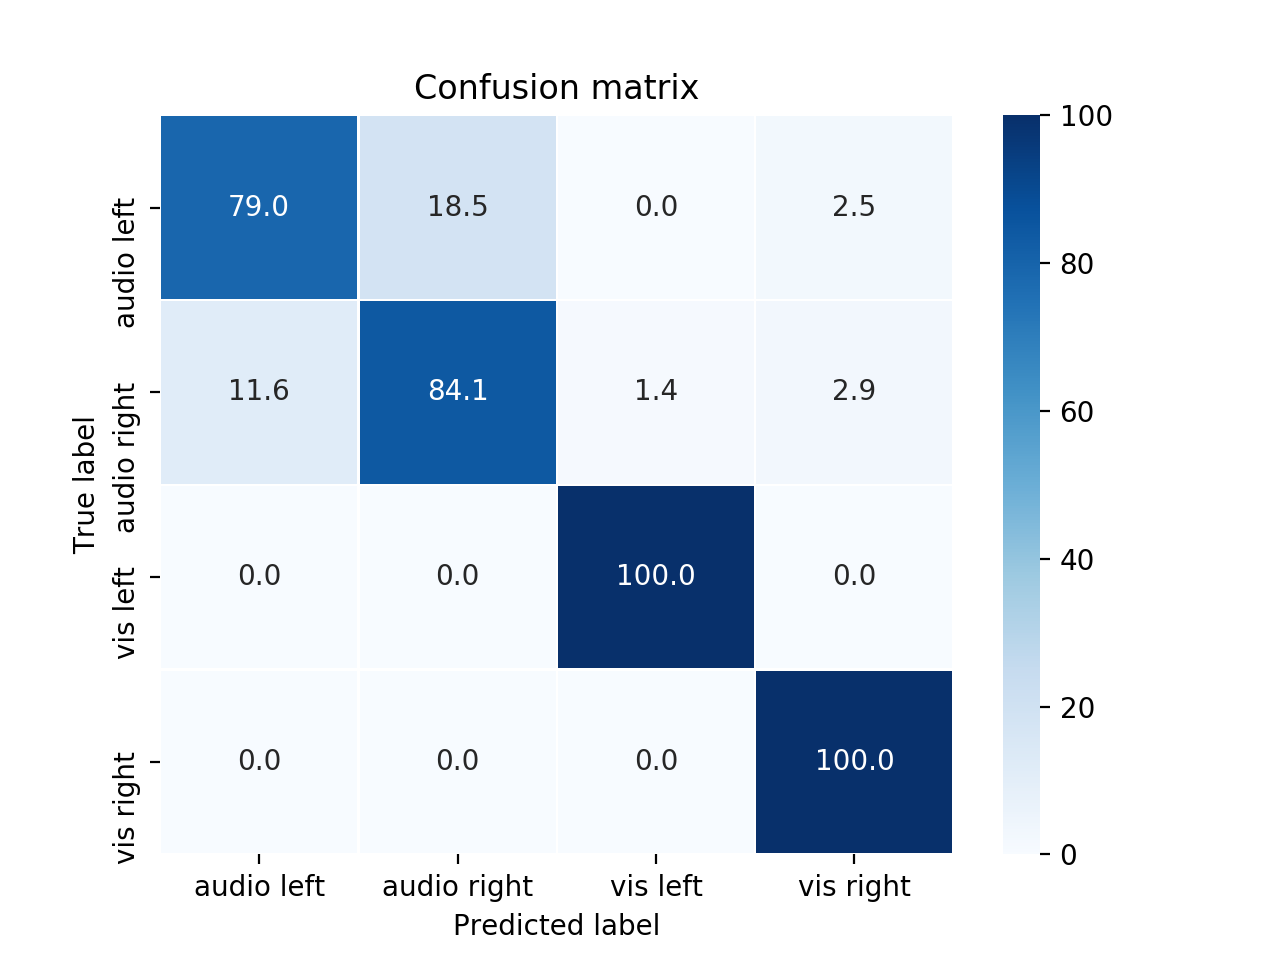
\includegraphics[width = 0.5\textwidth]{plot_classify_tangentspace.png}
        \end{center}

        \item Another classification method I found in their code used 
        an MDM (mean distance metric) algorithm, as discussed in their paper. 
        Upon running the python script \\
        plot\_classify\_MEG\_mdm.py, the code returned 
        \begin{center}
            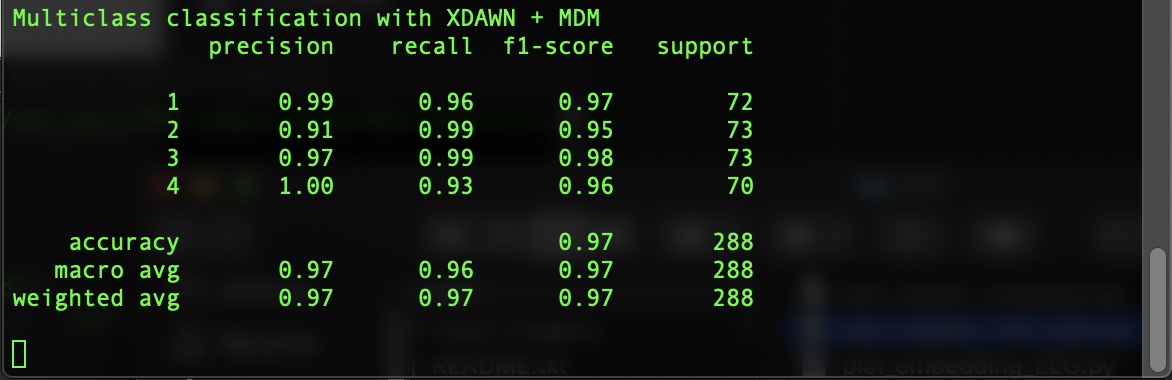
\includegraphics[width = 0.5\textwidth]{plot_classify_MEG_mdm2.png}
        \end{center}
        \begin{center}
            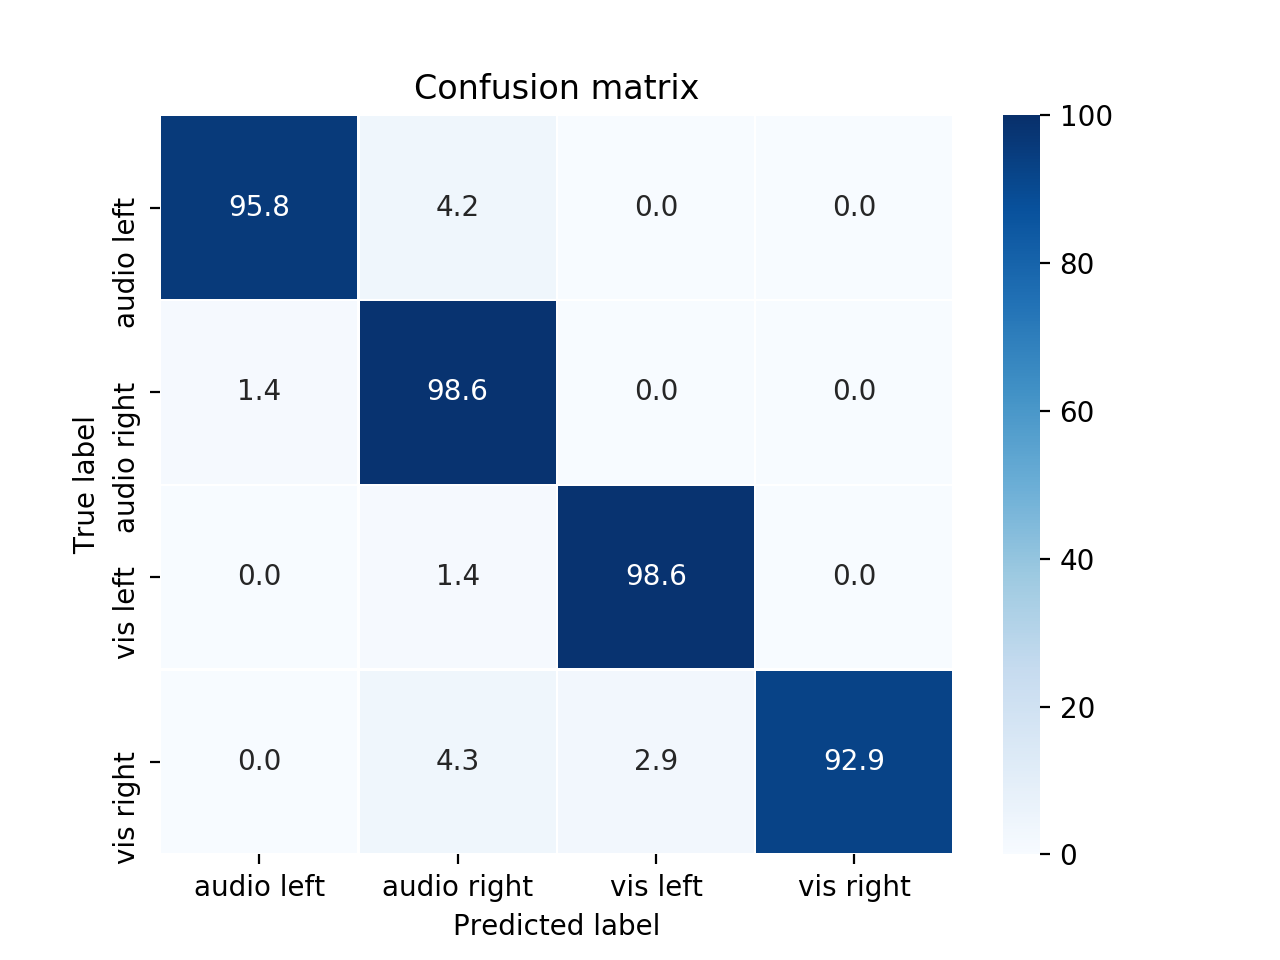
\includegraphics[width = 0.5\textwidth]{plot_classify_MEG1.png}
        \end{center}
        \begin{center}
            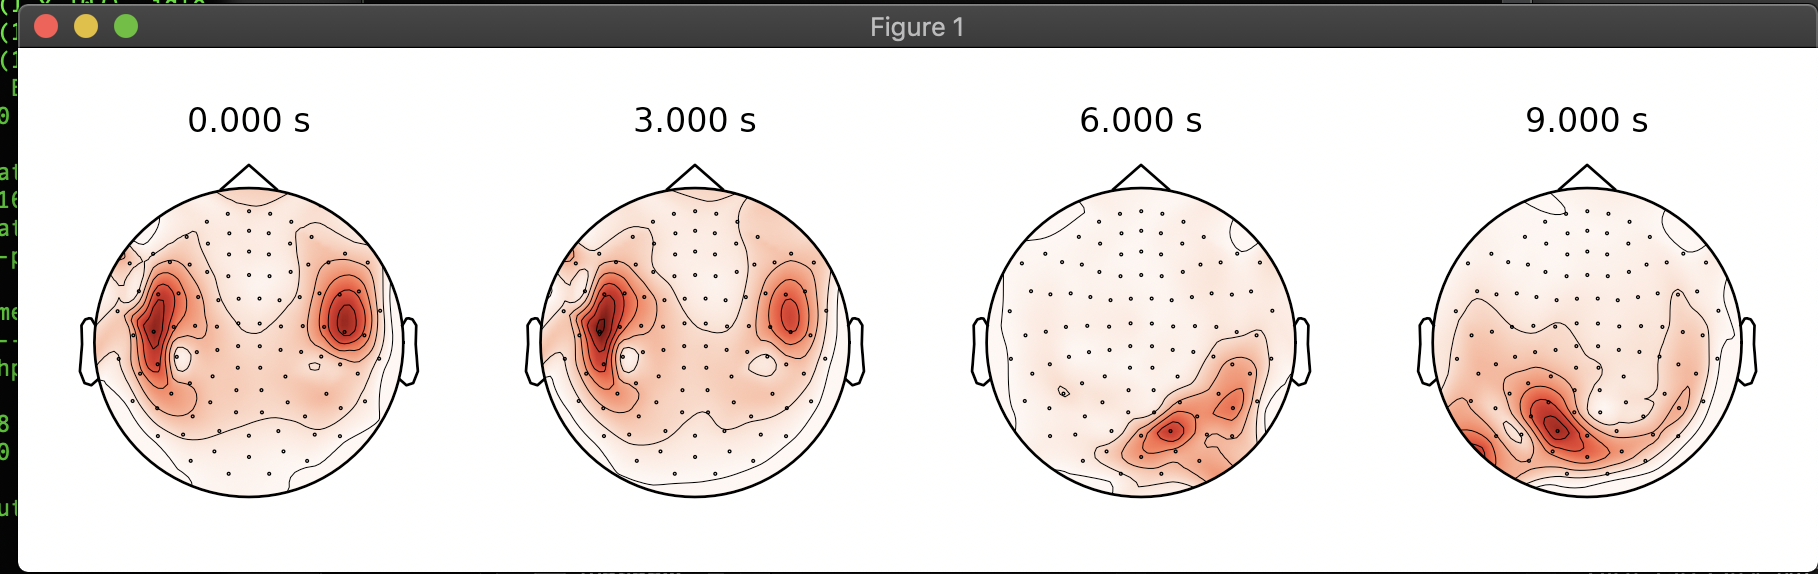
\includegraphics[width = 0.5\textwidth]{plot_classify_MEG_mdm3.png}
        \end{center}
        The above terminal output and confusion matrix reveals the accuracy of 
        their algorithms. I'm not quite sure what the third  

        \item The final script implemented in this example folder includes the  
        plot\_embedding\_EEG.py, which isn't discussed in their paper (and was probably just added later). 
        This returned a "spectral embedding."
        \begin{center}
            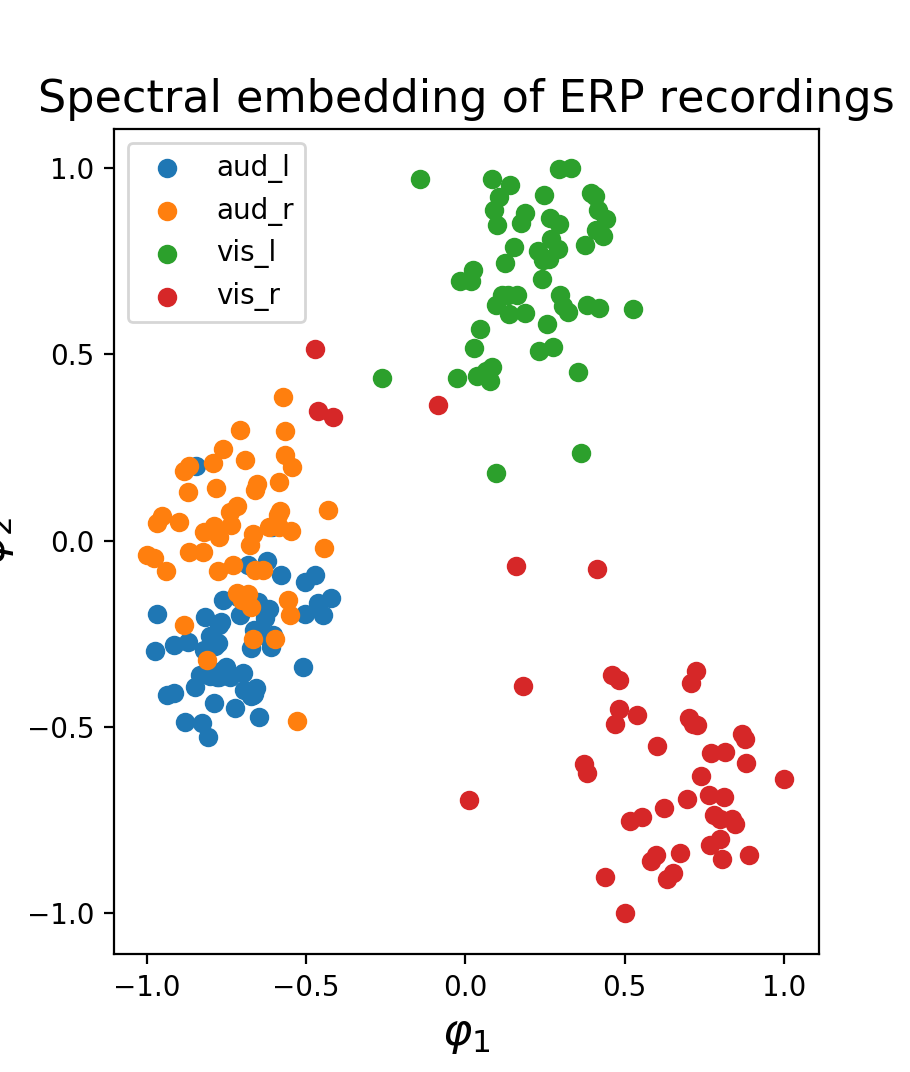
\includegraphics[width= 0.5\textwidth]{plot_embedding_EEG.png}
        \end{center}
    \end{itemize}
\end{solution}



\end{document}